\documentclass{article}

\usepackage[margin=1in]{geometry}
\usepackage{amsmath,amssymb}
\usepackage{graphicx}

\renewcommand{\thesection}{\arabic{section}}

\begin{document}

\title{Project AI \\ Auto-Encoding Stochastic Gradient Variational Bayes}
\author{	
	Joost van Amersfoort \\ 10021248  
	\and
	Otto Fabius \\ 5619858
	}
\maketitle

\begin{abstract}
In this paper, we implement and experiment with an auto-encoder trained with Stochastic Gradient VB \cite{kingma2013auto}. For each dataset, we learn the parameters for both an encoder and a decoder, implemented as two-layer neural networks, allowing for encoding data of the same type and generating new datapoints from (calculated or sampled) hidden representations. We use learned auto-encoders for generating new data and use the extracted features for classification. Several results from \cite{kingma2013auto} were reproduced and the results further show that the learned features generally improve classification accuracy.
\end{abstract}

\section{Introduction}

Before explaining what novelty was introduced by \cite{kingma2013auto}, it is first necessary to create some context and explain what an auto-encoder is, what it is used for and their current implementation. Auto-encoders, or autoassociators as \cite{bengio2009learning} calls them, are trained to encode the input in some representation so that the input can be reconstructed from that representation. In a simple network with one hidden layer that has a linear activation function and is trained with the mean squared error criterion, the hidden units learn the principal components of the data (PCA). However, if the hidden units have a non-linear activation function, the auto-encoder learns much more interesting things.

\cite{bengio2009learning} describe using auto-encoders as building blocks for a deep multi-layer neural network. 

\section{AEVB}

\subsection*{Problem class}

The problem class associated with AEVB is that where data $\mathbf{X}$ is assumed to be produced by some underlying process involving (continuous) hidden variables $\mathbf{Z}$. We can express the posterior probability over $\mathbf{X}$ by reformulating Bayes' Rule:

\begin{align}
P(X) = \frac{P(X|Z)P(Z)}{P(Z|X)}
\end{align}

Where $P(X|Z)$ and $P(Z|X)$ are parameterized by $\theta$.
\\

Knowing the probability distributions $P(X|Z)$ and $P(Z|X)$, i.e. learning $\theta$, can sometimes provide information on some natural process (if one is interested in the values of the parameters, for example). But knowing the distribution $P(Z|X)$ also allows us to infer $\mathbf{Z}$ from $\mathbf{X}$ to reduce the dimensionality of (encode) our data and find structure in the data. Furthermore, introducing a prior $P(Z)$ allows for computing the marginal probability $P(X)$ to generate data for applications such as image inpainting, denoising and super-resolution.
We would like to learn $\theta$ by gradient ascent/descent by differentiating some objective w.r.t. $\theta$. This can be done by choosing the marginal likelihood $P(X) = \int \frac{P(Z)}{P(X|Z)}dZ$ as objective to maximize, or by using the EM algorithm on the posterior density $ P(Z|X) = \frac{P(X|Z)P(Z)}{P(X)}$. However, calculating either  the marginal likelihood or the posterior density becomes intractable as the likelihood function $P(X|Z)$	 becomes more complex, which severely limits these methods. (possible e.g. variational linear regression, Bishop p. 486)





%In the class of problems we are interested in, the following conditions apply:
%\begin{itemize}
%\item The posterior distribution $P(Z|X)$ is intractable. 
%\item the probability density functions of the prior $P(Z)$ and the likelihood $P(X|Z)$, respectively, are differentiable w.r.t. $\mathbf{Z}$ and $\theta$. 
%\end{itemize}

\subsection{Sampling to obtain gradients}

Introducing $q(Z|X)$, parameterized by $\phi$, as an approximation of the posterior $P(Z|X)$, \cite{kingma2013auto} derive an expression for the Monte Carlo estimate of the lower bound $\mathcal{L}$ of the marginal likelihood $P(X)$:

\begin{align}
\mathcal{L}(\theta ,\phi ,  \mathbf{x^{(i)}}) \backsimeq \frac{1}{L} \sum_{l=1}^{L} \text{log } p_{\theta} (x^{(i)}|z^{(l)})+ \text{log }p(z^{(l)}	)-\text{log }q_{\phi}(z^{(l)}|x^{(i)})
\end{align}

Here, $z$ is sampled $l$ times from $q_{\phi}(z|x)$ for each datapoint $x^{(i)}$. Because $z$ therefore depends on parameters $\theta$, differentiating $\mathcal{L}$ w.r.t. $\phi$ will lead to a gradient which is influenced by the current parameters $\phi$. 
As a solution to this problem, \cite{kingma2013auto} reparameterize the samples of $z$ from $q(z|x)$ as
\begin{align}
z = g_\phi(\mathbf{\epsilon},\mathbf{x}) \text{  with  } \mathbf{\epsilon} \sim p(\mathbf{\epsilon}) 
\end{align} 

Now, once we have a sample $\epsilon$, the MC-estimate of $\mathcal{L}$ (equation (1) ) does not depend on a \textit{sampled} $z$, but on a  $z$ which is \textit{calculated deterministically}, independent of $\phi$. Thus, $\mathcal(L)$ can now be differentiated w.r.t all the parameters $\theta$ and $\phi$, enabling parameter optimization by means of stochastic gradient ascent.

\subsection{Modelling the conditional distributions}

For our experiments, we approximate $P(X|Z)$ and $q(X|Z)$ as neural networks with a single hidden layer, similar to \cite{kingma2013auto}. These neural networks can be trained well with backpropagation of error derivatives. They are also powerful, in the sense that they are universal approximators, i.e. they can approximate any function of their input. 

IETS OVER BINARY/CONTINUOUS OUTPUT \\
IETS MEER OVER NEURAL NETWORKS OID? IIG REFS...

This way, once we have trained the two networks, we have an \textit{encoder} that maps $\mathbf{x}$ to its hidden variables $\mathbf{z}$, and a (generative) \textit{decoder} that maps any combination of hidden variables to a (new) datapoint $\mathbf{x}$. This has a strong similarity to auto-encoders (refs??). 

The encoder allows us to compress and/or organize data. Inpainting, denoising and super-resolution (up to the resolution on which is trained) can be realized by generating the hidden representation from the datapoint with the encoder, and creating the desired output with the decoder.

\section{Experiments}

In this section, we outline our experiments and present our results. We will present and discuss our results immediately after the description of each experiment so it is clear to the reader which results and conclusion belong to which experiment.

\subsection{Reproducing results}

Firstly, we performed some experiments to reproduce the results of \cite{kingma2013auto}. This way, we can verify the correctness of our implementation. In their paper, an Auto-Encoder was trained on both binary valued data (MNIST handwritten digits) and continuous valued data (Frey Faces \footnote{Available at http://www.cs.nyu.edu/ ̃roweis/data.html}).

\subsubsection{MNIST}

We first trained an auto-encoder with 400 hidden units and 20-dimensional latent space with SGD-VB on MNIST, in order to compare the lower bound of the log likelihood with \cite{kingma2013auto}. Figure 1 shows the lower bound per data point during training for both the training set and the test set.  \\ 

\begin{figure}[htb]
\begin{center}
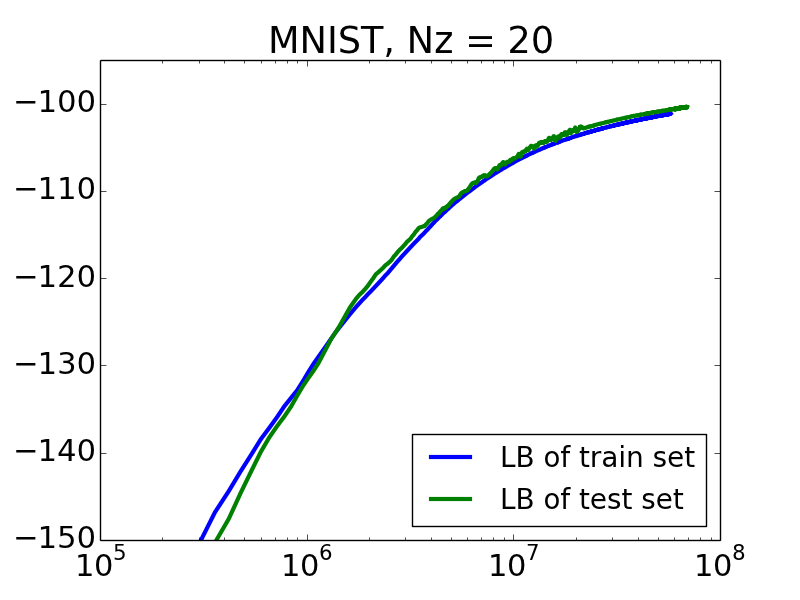
\includegraphics[height=3.1in,width=4in]{lowerboundAEVBMNIST.png}
\caption{Lower bound of the log likelihood per datapoint of both the train and test data during training. ...............}
\end{center}
\end{figure}

Also, we trained an auto-encoder with two-dimensional latent space in order to generate data for varying values of the latent variables along both latent dimensions. The resulting manifold is shown in Figure 2.

\begin{figure}[htb]
\begin{center}
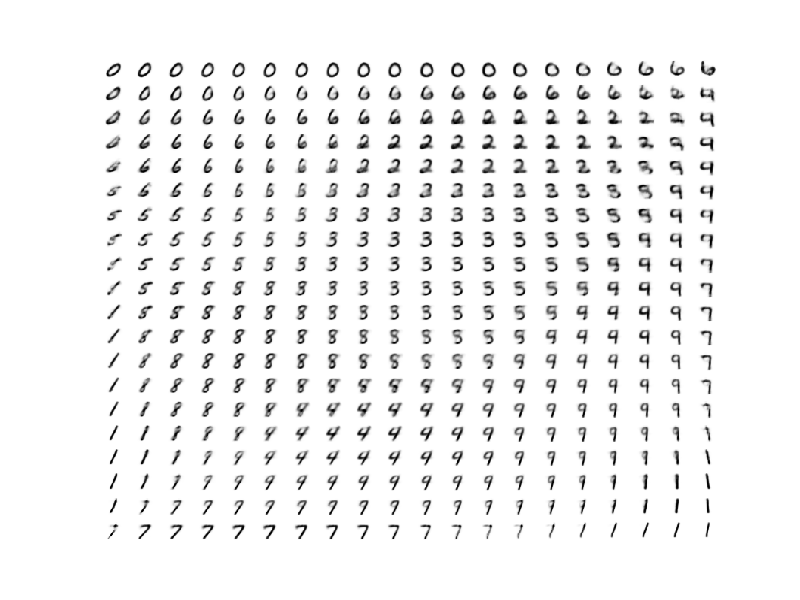
\includegraphics[height=4in,width=5in]{manifoldMNIST.png}
\caption{Visualization of generated data with two-dimensional latent space. Each datapoint was generated by calculating the mean outputs of the trained auto-encoder from a different hidden representation. The position in the total image reflects the coordinates of the hidden space and each image represents equal probability mass.}
\end{center}
\end{figure}

\subsubsection{Frey Faces}

Also for the continuous valued Frey Face dataset, we trained an auto-encoder with SGVB to compare the progression of the lower bound to that in \cite{kingma2013auto}. Figure 3 shows the lower bound of the training and test set as training progresses for latent dimensionality of 10, with 200 hidden units.

\begin{figure}[htb]
\centering
\begin{minipage}{0.5\textwidth}
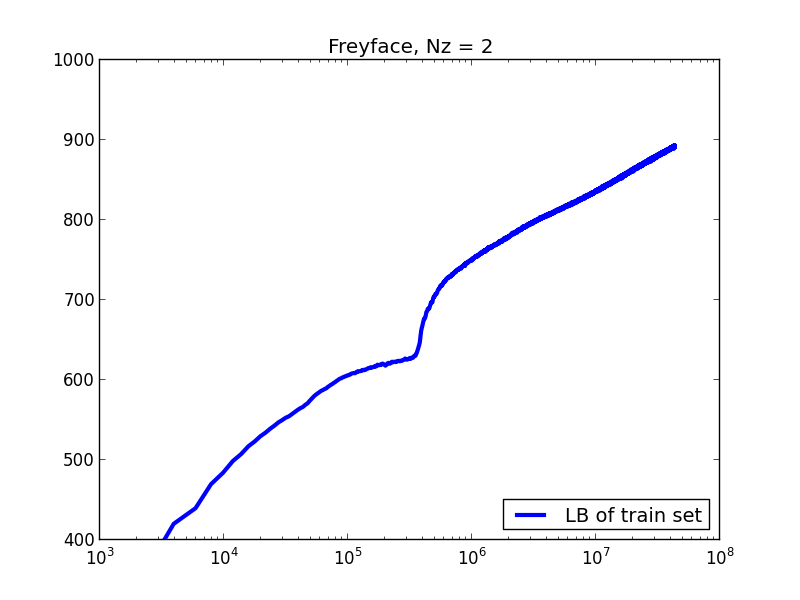
\includegraphics[height=3in,width=3.6in]{lowerboundFF.png}
\caption{...............}
\end{minipage}%
\centering
\begin{minipage}{0.5\textwidth}
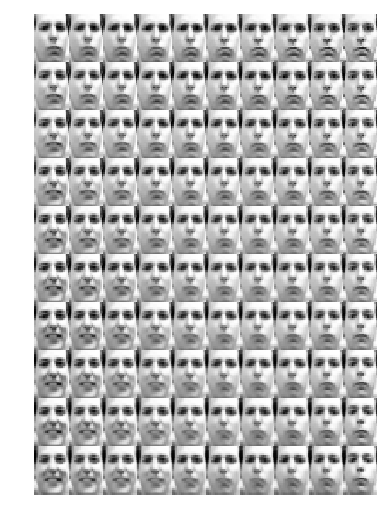
\includegraphics[height=3.2in,width=3.2in]{manifoldFF.png}\caption{...............}
\end{minipage}
\end{figure}

Training an auto-encoder with 200 hidden units and 2 latent dimensions once again enables visualization of generated data along both dimensions, shown in Figure 4.

These results achieved with our implementation of SGDVB auto-encoders are very similar to those to those presented in \cite{kingma2013auto}, which shows that our implementation is correct and that these results can be achieved consistently. 

\subsection{Classification}

In the remainder of the experiments, we will focus on one useful application of learned features, namely in classification. Before we use a classification method, we can use a trained Auto-Encoder to extract features from the data by calculating the output of the hidden layer of the Auto-Encoder. This way, we aim to improve the results of classification (supervised learning) with SGDVB (unsupervised learning). In particular, we will examine the performance of logistic regression on various representations of the same dataset. Classifying on features calculated by a one-layer neural network effectively results in a two-layered MLP, of which the first layer is not trained with supervised learning after training it with SGDVB. We compare obtained results to those obtained when using features trained with a Restricted Bolzmann Machine, which is a popular method for such (??) feature extraction and is frequently used for weight initialization in layers of deep belief nets (e.g. \cite{bengio2007greedy} ).

\subsubsection{Classifying MNIST on features}

In this subsection, we detail how well logistic regression performed on MNIST when using raw pixel data as input, features learned with an SGDVB Auto-Encoder as input, and with features learned with an RBM as input. \\ For this, we used the same Auto-Encoder of which the lower bound is shown in Figure 1. Thus, it has 400 hidden units and latent dimensionality of 20, was trained on approximately $5.0\cdot 10^7$ training examples, and reached a lower bound of $-101.53$ on the log likelihood per data point. The trained RBM also contained 400 hidden units to ensure the same representational power, and was trained on $1.5\cdot 10^7$ training examples from the MNIST training set. This yielded the same results as $0.5\cdot 10^7$ training examples and thus was enough iterations for convergence.\\
Logistic regression was run until results on the validation set declined or stabilized. The results are shown in Table 1.

\begin{table}
\begin{tabular}{|l|c|c|r|}
\hline
& Raw Data & SGVB AE Features & RBM Features \\ \hline
No. of training examples until convergence ($\cdot 10^6$) & 1.5 & 4.0 & 3.0 \\ \hline 
Test set accuracy & 93.36 & 97.54 & 96.29
\end{tabular}
\end{table}

As expected, using features calculated with the trained RBM improved the test set accuracy. However, the results using the trained auto-encoder were even better, leading to an error rate of only 2.46\%! This is an important finding, as auto-encoding SGVB proves to be a at least viable alternative to using an RBM for unsupervised learning. Besides outperforming RBM's (at least for this task), AE SGVB is theoretically more attractive than RBM's as it has a clearer objective that is maximized, and allows for calculating the lower bound, allowing for (efficient) monitoring during optimization and comparison  of lower bound across various parameter settings.\\
As the features were extracted from a one-layer neural network, this result was effectively achieved with a two-layer neural network, and it compares well to the 'classic' results achieved with two-layer NNs by \cite{lecun1998gradient}, who was only able to further improve results by deskewing. In this experiment, the first layer was not trained beyond unsupervised learning. Training both layers of the neural network during supervised learning could therefore further improve results.

\subsubsection{Classifying Chinese characters}

To investigate whether the boost in classification accuracy generalizes (at least in part) to other data, we also performed classification on the handwritten Chinese character dataset (voetnote, referentie of iets). \\
This dataset consists of 1,121,749 annotated datapoints in 3,750 different classes, with each class containing approximately the same number of characters. Each datapoint contains grey values of an image of a handwritten Chinese character and a code for its corresponding class. For preprocessing, we binarized the images and scaled them to 40x40. This is still larger than MNIST, which has dimensions 28 x 28 but was deemed necessary to keep the more fine grained structure of the characters intact. As images had varying aspect ratios, we added white padding whenever necessary, in order to have constant dimensionality of the data. Due to resource and time limitations, we only used 50 classes, resulting in 11,578 data points. The resulting dataset is similar to MNIST in size and type, but considerably more complex in that the images are larger, there are 5 times as many classes, and the structure in the images is more complex.\\
Once again, we trained an auto-encoder on the data, and used logistic regression to classify the data. For the auto-encoder, we used 500 hidden units and hidden dimensionality of 200. The auto-encoder is trained on the 10,000 images in the train set and the lower bound on the log likelihood during training is shown in Figure 5. 

\begin{figure}[htb]
\begin{center}
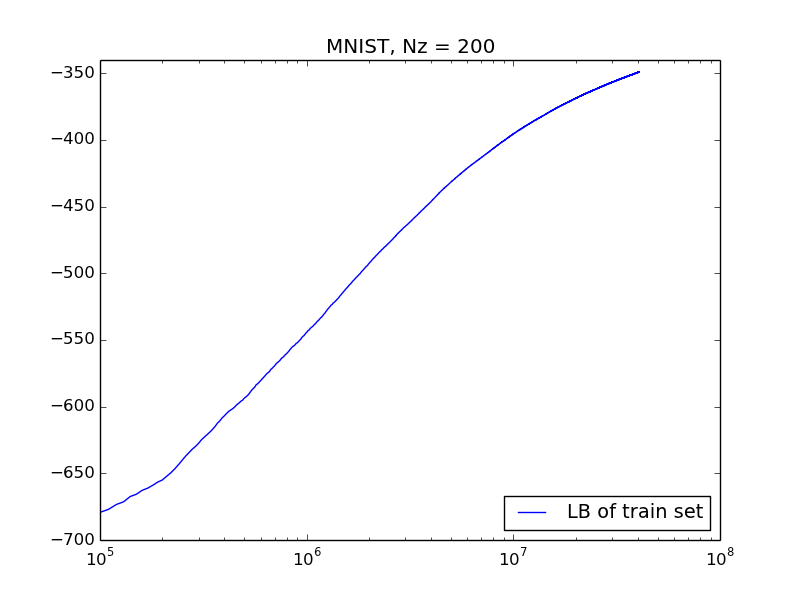
\includegraphics[height=3.1in,width=4in]{lowerboundchinese.png}
\caption{Lower bound of the log likelihood per datapoint of the train set during training.}
\end{center}
\end{figure}

Once again, we trained a classifier with logistic regression on both the preprocessed pixel values as well as the features extracted from the trained encoder. Logistic regression on the pixel values yielded a test set accuracy of 66.29\%, compared to 69.17\% when classifying on the features. Percentage-wise, this is a similar increase in accuracy as achieved on MNIST, but as the scores are much lower than on MNIST, this increase is relatively small. It is not obvious whether this indicates whether  One possible explanation is that 



\subsubsection{Classification on small datasets}

In practice it is hard to obtain large annotated datasets for supervised learning. Therefore, we also tested the effectiveness of features calculated from a trained Auto-Encoder for improving the classification results for small subsets of MNIST (and Tsaie Niis characters?). Once again, logistic regression is our classification method of choice. \\ In our experiment, we selected the first $x$ training examples from the training set of MNIST as our training set, where $x$ started at 4 and was increased each time by multiplying it with 2, up to a size of 2048. To evaluate the results for each dataset size, we took the first 1000 datapoints of the MNIST test set.

\section*{Conclusion}



\pagebreak 
\section*{References}
\bibliographystyle{amsplain}
\bibliography{references}

\end{document}
